%%%%%%%%%%%%%%%%%%%%% Chapter 15 %%%%%%%%%%%%%%%%%%%%%%%%%%%%%%%%%
% Efficient AI: Trustworthy Quantization & Pruning
%%%%%%%%%%%%%%%%%%%%%%%%%%%%%%%%%%%%%%%%%%%%%%%%%%%%%%%%%%%%%%%%%
\motto{If a privacy-preserving model cannot run on a standard smartphone or IoT device, it remains a laboratory experiment. Efficiency is not optional; it is a prerequisite for trustworthy deployment.}

\chapter{Efficient AI: Trustworthy Quantization \& Pruning}
\label{chap:efficient_ai}

\abstract{This chapter explores the critical intersection between trust and performance. While defenses like Differential Privacy and Secure Aggregation provide robust protection, they often impose significant computational and communication overhead. We analyze how to make these "heavy" defenses practical through model compression, quantization, and pruning. By moving inference to the edge and reducing the multi-party communication burden, efficient AI enables the large-scale adoption of trustworthy technologies in resource-constrained environments like ASEAN.}

\section{Privacy Requires Efficiency}
\label{sec:privacy_efficiency}

As we have seen in the preceding parts of this book, building a trustworthy system is computationally expensive. Differential Privacy requires per-sample gradient clipping and noise injection; Secure Aggregation requires multiple cryptographic rounds and key exchanges; and robust models often require larger architectures to maintain accuracy under noise.

If these models are too heavy to run on the consumer devices (smartphones, IoT sensors) where data is actually generated, architects are forced to move processing to the cloud, re-introducing the privacy risks we seek to avoid. For the Trustworthy AI Architect, efficiency is the enabling pillar that makes decentralized privacy a reality.

\section{Core Efficiency Techniques}
\label{sec:efficiency_techniques}

To reduce the footprint of a model while maintaining its trustworthiness, we employ three primary technical maneuvers derived from foundational compression research \cite{han2015}:

\begin{description}
  \item[Quantization:] 
        Reducing the numerical precision of model weights and activations (e.g., from 32-bit floating point to 8-bit integers). This dramatically reduces memory usage and speeds up inference with minimal loss in accuracy.
        \begin{equation}
        x_{int} = \text{round}\left(\frac{x_{fp}}{\text{scale}} + \text{zero\_point}\right)
        \end{equation}
  \item[Pruning:]
        Identifying and removing redundant neurons or synaptic connections that contribute little to the model's final prediction. \textit{Magnitude pruning} is a common heuristic:
        \begin{equation}
        \text{mask}_i = \begin{cases} 1 & \text{if } |w_i| > \text{threshold} \\ 0 & \text{otherwise} \end{cases}
        \end{equation}
  \item[Knowledge Distillation:]
        Training a smaller, "student" model to mimic the outputs and behavior of a larger, "teacher" model. This allows for the deployment of a lightweight architecture that retains much of the knowledge and robustness of a massive ensemble.
\end{description}

\begin{figure}[t]
\centering
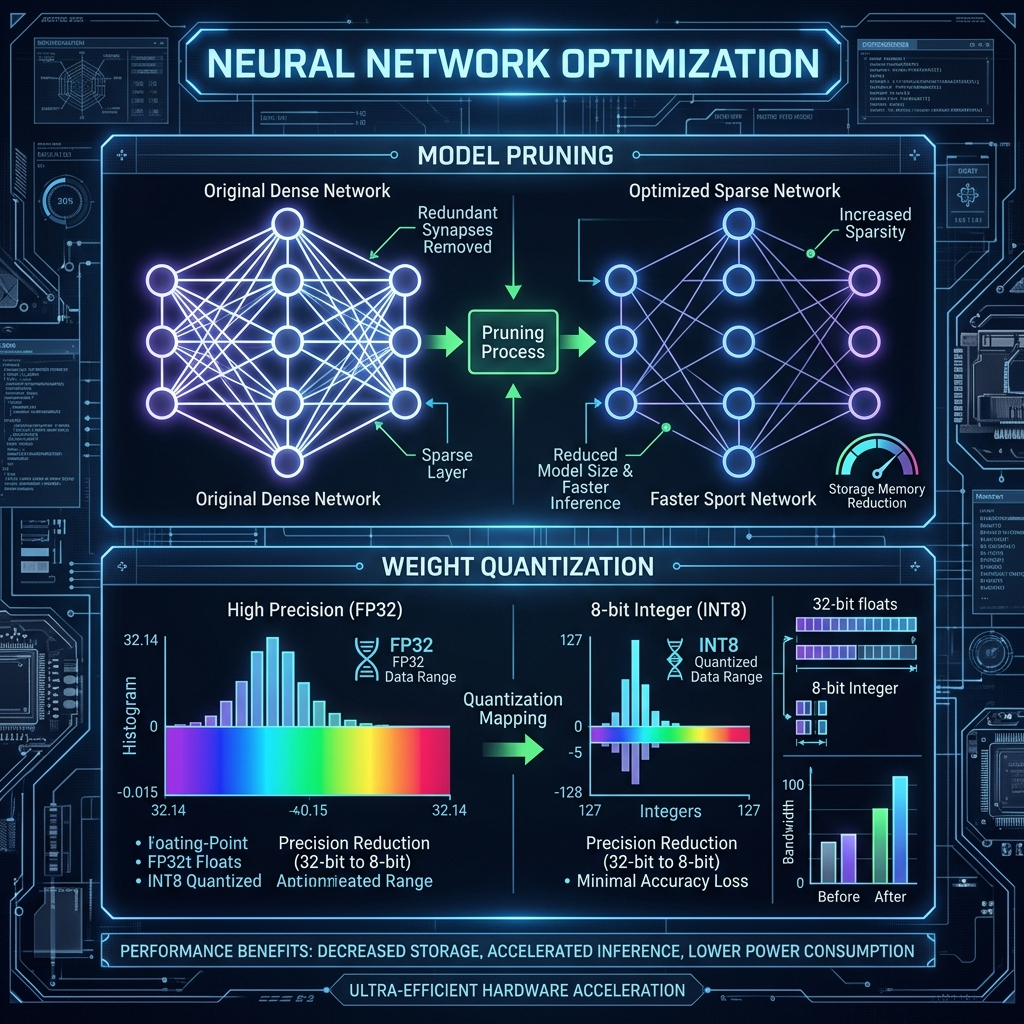
\includegraphics[width=\textwidth]{figures/ch14_optimization.png}
\caption{Model Optimization for Trustworthy AI: Comparing the mechanisms of Neural Network Pruning and Weight Quantization to enable privacy-preserving deployment on edge devices.}
\label{fig:ch14_optimization}
\end{figure}

\section{Neural Architecture Search (NAS)}
\label{sec:nas}

For high-end edge deployments, architects can use \textbf{Neural Architecture Search (NAS)} to automatically discover the optimal model structure for a specific hardware target. The objective is to minimize validation loss while respecting a strict latency or memory constraint:
\begin{equation}
\min_{\text{arch}} L_{\text{val}}(\text{arch}, w^*) \quad \text{s.t. } \text{Latency}(\text{arch}) \le T_{\text{max}}
\end{equation}

\section{Sustainable AI: Excellence through Energy Efficiency}
\label{sec:sustainable_ai}

In the 2026 technical landscape, the role of the Trustworthy AI Architect has expanded to include environmental accountability. As we have seen, privacy-preserving defenses add significant computational overhead. To satisfy the mandate of \textbf{Sustainable AI} \cite{schwartz2020} (aligned with Vietnam's 2026 carbon neutrality strategy), we must move beyond pure accuracy toward energy-aware optimization.

The "Carbon-Aware Architect" optimizes models using two primary metrics:
\begin{itemize}
    \item \textbf{Power Usage Effectiveness (PUE):} Ensuring that the infrastructure supporting the AI (data centers, edge clusters) is optimized for thermal and electrical efficiency.
    \item \textbf{FLOPs-per-Watt:} A specialized efficiency metric that measures the amount of intellectual work (Floating Point Operations) performed per unit of energy consumed.
\end{itemize}

\subsection{Green-by-Design Lifecycle}
To build sustainable trust, architectures must prioritize \textbf{Green-by-Design} principles. This includes using \textit{Conditional Computation} (only activates specific neural pathways when needed) and \textit{Carbon-Intelligent Scheduling} (performing heavy training or batch inference during hours when the local grid's renewable energy supply is at its peak). By optimizing for the "Watt" as well as the "Bit," the architect ensures that AI remains a tool for long-term societal benefit rather than an ecological burden.

\section{Conclusion}
\label{sec:conclusion_efficiency}

Part IV has addressed the internal properties of our systems: their robustness to adversarial input, their transparency to human operators, and their practical efficiency on the edge. By integrating sustainability into our efficiency stack, we align our technical goals with global accountability standards. However, building these hardened models is only half the battle. We must also ensure they are accountable to the creators of their training data. In the next chapter, we address the unique challenges of \textbf{Intellectual Property and Deepfake Defense} in the age of generative media.


